\section{پیش‌بینی پیوند داخل انجمن‌ها}

ایدهٔ استفاده از اطلاعات انجمن‌ها برای کمک به روش‌های پیش‌بینی پیوند، پیش از این در کار ساندراجان\LTRfootnote{Soundarajan} و هاپکرفت\LTRfootnote{Hopcroft} \cite{soundarajan2012using} استفاده شده بود. آن‌ها تعریف شاخص‌های شباهت را تغییر داده بودند و اطلاعات انجمن‌ها را در آن وارد کرده بودند و نتیجه گرفته بودند که در بیشتر مواقع، این شاخص‌های جدید گسترش‌یافته، می‌توانند از شاخص‌های معمولی کارایی بهتری از خود نشان دهند.

در این پژوهش، ایده اصلی این است که در بیشتر موارد، پیوندهای بالقوه درون انجمن‌ها بسیار کمتر از پیوندهای بالقوه بین انجمن‌ها هستند. این موضوع با یک مثال ساده روشن‌تر می‌شود. فرض کنید یک شبکه داریم که از ۱۰۰ گره تشکیل شده‌است. این شبکه درون خود دارای ۵ انجمن است که هر کدام از این انجمن‌ها ۲۰ گره درون خود دارند. بنابر این تعداد کل پیوندهای بالقوه درون کل انجمن‌ها این شبکه برابر خواهد بود با ۵‫×‬۲۰‫×‬۱۹ که برابر است با ۱۹۰۰ یال بالقوه. اما از سوی دیگر تعداد کل پیوندهای بالقوه بین انجمن‌ها برابر خواهد بود با ۵‫×‬۲۰‫×‬۸۰ که برابر است با ۸۰۰۰ یال بالقوه. همان‌طور که مشاهده می‌شود، تعداد یال‌های بالقوه داخل انجمن‌ها بسیار کمتر از تعداد یال‌های بالقوه بین انجمن‌ها خواهد بود. همچنین، در بیشتر موارد، چگالی یال‌های داخل یک انجمن بیشتر از چگالی یال‌های بیرون از انجمن‌ها است، به این دلیلِ بدیهی که تعریف «انجمن» این‌گونه حکم می‌کند. یعی برای مثال درصد بسیار بیشتری از ۱۹۰۰ یال بالقوه یادشده داخل انجمن‌ها در واقع موجودند تا ۸۰۰۰ یال بالقوه بیرون از انجمن‌ها.

این ایده‌ها کمک می‌کنند تا بتوان به روش مناسبی دست پیدا کرد. بنا بر بحث‌های بالا، محدود کردن پیش‌بینی پیوند به پیش‌بینی درون انجمن‌ها، کمک خواهد کرد تا بتوان پیوندهای درست بیشتری را تشخیص داد. دلیل این امر این است که یک گره، با احتمال بیشتری با یک گره از انجمن خود پیوند برقرار می‌کند تا یک گره از بیرون انجمن‌ خود. البته طبیعی است که با این کار پیش‌بینی پیوندهای بالقوه بین انجمن‌ها را از دست خواهیم داد، اما در تعداد محدودی پیش‌بینی، این کار می‌تواند به افزایش دقت پیش‌بینی‌های ما کمک شایانی بکند.

\subsection{تعریف ریاضی روش}
برای ارائه تعریف ریاضی دقیق‌تر برای این روش‌ها، فرض کنید یک شبکه داریم که قصد داریم در آن پیش‌بینی پیوند انجام دهیم. ابتدا شاخص شباهت مورد نظر خود (برای مثال شاخص همسایه‌های مشترک) را روی شبکه محاسبه می‌کنیم. همچنین به طور موازی یک روش تشخیص انجمن را نیز بر روی شبکه مورد نظر خود اجرا می‌کنیم تا انجمن‌های موجود در شبکه را بشناسیم. فرض کنید که $SM(x,y)$ مقدار شاخص شباهت مورد نظر بین دو گره $x$ و $y$ باشد. رابطهٔ محاسبهٔ روش پیشنهادی به صورت زیر خواهد بود:
\begin{equation}\label{SMxCO}
  SM'(x,y)=SM(x,y) \times CO(x,y),\\
\end{equation}
که در آن، CO به صورت زیر تعریف می‌شود:
\begin{equation}
  CO(x,y)=  \left\{
              \begin{array}{rcl}
                1 & \text{if} & comm(x) = comm(y) ,\\
                0 & \text{if} & otherwise.
              \end{array} \right.
\end{equation}
و مقدار $comm(x)$ به انجمنی اشاره دارد که شامل گره $x$ می‌شود.

همان‌طور که از رابطه \ref{SMxCO} مشخص است، پس از محاسبهٔ شاخص شباهت و تشخیص انجمن‌های شبکهٔ مورد نظر، مقدار نهایی روش پیشنهادی یعنی $SM'$، شاخص شباهت اصلی را فقط بین گره‌هایی که در یک انجمن یکسان حضور دارند مورد توجه قرار می‌دهد و بین بقیهٔ جفت گره‌هایی که در یک انجمن یکسان نیستند، مقدار صفر به خود می‌گیرند. بنابراین در این‌جا در واقع پیش‌بینی پیوند داخل انجمن‌ها انجام می‌گیرد که در بخش قبل  نیز به آن اشاره شد.

\subsection{استفاده از وزن پیوندها}
همان‌طور که در بخش‌های قبل نیز به آن اشاره شد، در بسیاری موارد اطلاعات مفید دیگری نیز در شبکه‌ها وجود دارند که می‌توانند به بهبود کارایی و افزایش دقت روش‌های پیش‌بینی پیوند کمک کنند. یکی از این اطلاعات ارزشمند، وزن پیوندهاست. همان‌طور که از عنوان این پژوهش نیز بر می‌آید، قصد آن این است که بتواند روش‌های پیش‌بینی پیوند را با کمک گرفتن از وزن پیوندها بهبود ببخشد و دقت پیش‌بینی‌ها را افزایش دهد.

با توجه روشی که در بخش گذشته پیشنهاد شد، این روش از دو گام مجزا تشکیل شده‌است. گام اول محاسبهٔ معیارهای شباهت بین هر دو گره دلخواه در شبکه که پیوندی بین آن دو وجود ندارد؛ و گام دوم تشخیص انجمن‌ها در همان شبکه، که در نهایت با ترکیب این دو گام نتیجهٔ نهایی به دست می‌آید. بر طبق توضیحاتی که در قسمت‌های قبل داده شد، هر دوی این گام‌ها می‌توانند از وزن پیوندها استفاده کنند. در گام اول یعنی محاسبهٔ معیارهای شباهت، در بخش \ref{subsec:similarity} برای هر کدام از شاخص‌ها گسترش آن‌ها به حالت وزن‌دار نیز بررسی شد و با استفاده از روابط موجود می‌توان آن‌ها را در حالت وزن‌دار محاسبه کرد. در گام دوم یعنی تشخیص انجمن‌ها نیز همان‌طور که گفته شد، الگوریتم \Infomap دارای حالت وزن‌دار است و می‌تواند از شبکه ورودی وزن‌دار استفاده کرده و انجمن‌ها را با استفاده از آن تشخیص دهد.

همان‌طور که عنوان شد، در روش پیشنهادی دو گام محاسبهٔ شاخص و تشخیص انجمن وجود دارد که هر بخش می‌تواند بدون وزن یا وزن‌دار انجام گیرد. در نتیجه با توجه به این که در هر کدام از این دو بخش، کدام حالت (یعنی بدون وزن یا وزن‌دار) را انتخاب کنیم، روش‌های پیشنهادی به چهار روش گسترش داده می‌شود:

{ \onehalfspacing
\begin{enumerate}
  \item محاسبهٔ شاخص بدون وزن همراه با تشخیص انجمن بدون وزن
  \item محاسبهٔ شاخص بدون وزن همراه با تشخیص انجمن وزن‌دار
  \item محاسبهٔ شاخص وزن‌دار همراه با تشخیص انجمن بدون وزن
  \item محاسبهٔ شاخص وزن‌دار همراه با تشخیص انجمن وزن‌دار
\end{enumerate}
}
جدول \ref{tab:3-1} این تقسیم‌بندی را نشان می‌دهد. همان‌طور که در این جدول نشان داده شده‌است، از این پس برای ارجاع دادن به هر کدام از این روش‌ها از علائم اختصاری آن‌ها استفاده می‌کنیم که به ترتیب عبارتند از:
\lr{UU}، \lr{UW}، \lr{WU} و \lr{WW}.

{ \def\arraystretch{2.0}
\begin{table}[!hb]
  \caption{چهار روش پیشنهادی برای استفاده از اطلاعات وزن پیوندها، و انجمن‌ها}
  \label{tab:3-1}

  \begin{center}
  %\renewcommand{\arraystretch}{2.0}
    \begin{tabular}{|m{3cm}|m{2cm}|p{4cm}|p{4cm}|}
      \cline{3-4}
      \multicolumn{2}{c|}{\multirow{2}{*}{}} & \multicolumn{2}{c|}{شاخص پیش‌بینی پیوند} \\ \cline{3-4}
      \multicolumn{2}{c|}{} &
        \multicolumn{1}{c|}{بدون وزن} &
        \multicolumn{1}{c|}{وزن‌دار} \\ \hline
      \multirow{2}{*}{روش تشخیص انجمن} &
        بدون وزن &
        ترکیب شاخص بدون وزن با تشخیص انجمن بدون وزن (شماره ۱) که با $ UU $ نمایش داده می‌شود &
        ترکیب شاخص وزن‌دار با تشخیص انجمن بدون وزن (شماره ۳) که با $ WU $ نمایش داده می‌شود \\ \cline{2-4}
      &
        وزن‌دار &
        ترکیب شاخص بدون وزن با تشخیص انجمن وزن‌دار (شماره ۲) که با $ UW $ نمایش داده می‌شود &
        ترکیب شاخص وزن‌دار با تشخیص انجمن وزن‌دار (شماره ۴) که با $ WU $ نمایش داده می‌شود\\ \hline
    \end{tabular}
  \end{center}
\end{table}
}

این چهار روش هر کدام می‌توانند با توجه به ساختار و ویژگی‌های شبکه‌های مختلف، در مجموعه داده‌های مختلف، متفاوت عمل کنند و کارایی‌های مختلفی از خود نشان دهند. هدف این پژوهش این است که این چهار روش را در حالت‌های مختلف شبکه‌ها بررسی کند و نشان دهد که هر کدام از آن‌ها در چه نوع شبکه‌هایی عملکرد خوبی از خود نشان دهند و از سوی دیگر در کدام نوع شبکه‌ها عملکرد مناسبی ندارند. همچنین دلیل عملکردهای متفاوت این روش‌ها نیز بررسی خواهد شد. برای مثال اگر در شبکه‌ای پیوند‌های بیرون انجمن‌ها قوی‌تر باشد، ممکن است روش تشخیص انجمن وزن‌دار به نتایج مناسبی ارائه ندهد و دقت پیش‌بینی را کم کند. به این موضوع در فصل بعد به تفصیل پرداخته خواهد شد.

% \begin{figure}
%   \begin{center}
%     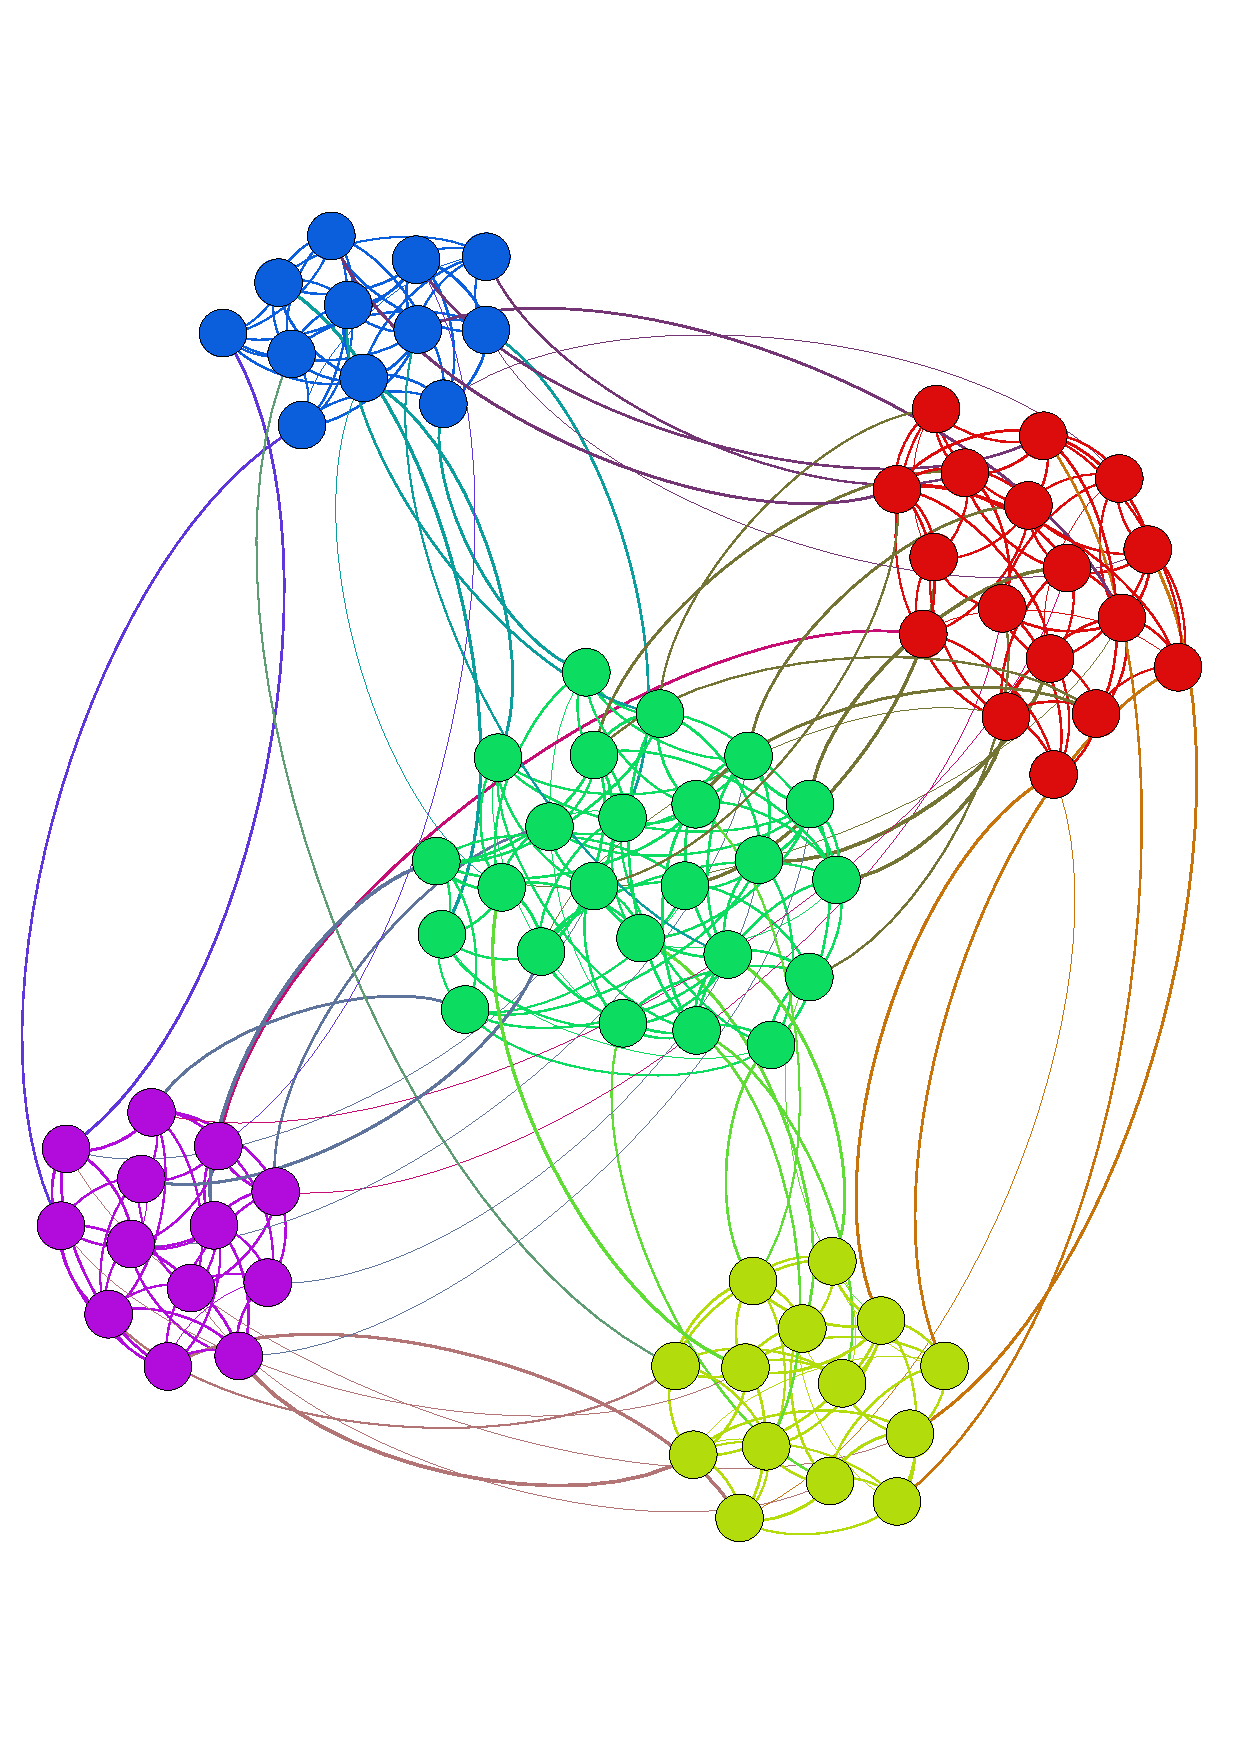
\includegraphics[width=10cm,height=10cm,keepaspectratio]{80.pdf}
%     \caption{}
%     \label{fig:}
%   \end{center}
% \end{figure}

\subsection{رویکرد عملی محاسبهٔ شاخص‌های پیشنهادی}\label{subsec:practical}
با وجود این که در بخش قبل یک تعریف ریاضی از نحوهٔ محاسبهٔ روش‌ها ارائه شد، اما می‌توان از رویکرد دیگری نیز برای محاسبهٔ آن‌ها استفاده کرد. البته باید توجه داشت که نتایج این رویکرد جدید محاسبه ممکن است در مواردی با نتایج رویکرد ریاضی که در رابطهٔ \ref{SMxCO} معرفی شد متفاوت باشد. در رویکرد قبلی، گام تشخیص انجمن به طور موازی با گام محاسبهٔ شاخص شباهت انجام می‌شد و در نهایت نتایج این دو گام با هم ترکیب می‌شدند. اما در این رویکرد گام تشخیص انجمن می‌تواند ابتدا انجام شود، سپس شبکه مورد نظر به انجمن‌های خود شکسته شود و در گام بعد، برای هر انجمن محاسبهٔ شاخص شباهت به طور مجزا انجام گیرد. برتری این رویکرد نسبت به رویکرد قبلی در این نکته است که مرتبهٔ\footnote{\lr{order}} انجمن‌های یک شبکه به مراتب از خود شبکه کمتر است. با توجه به این که پیچیدگی زمانی\footnote{\lr{time complexity}} برای بیشتر روش‌ها طبق آن‌چه که در \cite{wang2015link} عنوان شده است، از $O(n^2)$ (و ضرایب آن) است\footnote{به جز شاخص \textit{«وابستگی ترجیحی»} که پیچیدگی زمانی آن از مرتبهٔ $O(n)$ است.}، این امر باعث می‌شود که از پیچیدگی زمانی فرآیند محاسبهٔ شاخص‌های شباهت کاسته شود.

برای روشن‌تر شدن موضوع یک مثال بسیار ساده ارائه می‌شود: فرض کنید یک گراف با ۵۰۰۰ گره داریم که دارای ۱۰۰ انجمن با میانگین تعداد اعضای ۵۰ است. برای محاسبهٔ هر یک از شاخص‌های شباهت (که پیچیدگی زمانی از مرتبه $O(n^2)$ دارند) برای مثال معیار \textit{«همسایه‌های مشترک»} لازم است که محاسباتی از مرتبهٔ
$5\,000^2 = 25\,000\,000$
انجام شود. اما اگر از رویکرد دوم برای محاسبه استفاده کنیم، محاسبات ما از مرتبهٔ
$100 \times 50^2 = 250\,000$
خواهد بود که بسیار کمتر از روش محاسبه‌‌ٔ اول است.

البته همان‌طور که گفته شد باید توجه داشت که خروجی در این حالت با خروجی حالت قبل ممکن است متفاوت باشد. دلیل این امر نیز این است که اگر دو گره که عضو یک انجمن هستند همسایهٔ مشترکی خارج از انجمن داشته باشند، در معیارهایی که بر پایهٔ همسایه‌های مشترک استوارند (مانند \textit{همسایه‌های مشترک}، \textit{آدامیک/ادار}، \textit{تخصیص منابع} و…)، با استفاده از رویکرد جدید، این همسایهٔ مشترک محاسبه نمی‌شود و همین امر منشأ تفاوت بین خروجی‌ها خواهد بود. اما در روشی مثل \textit{وابستگی ترجیحی} این مشکل وجود نخواهد داشت و نتیجه در دو حالت یکسان خواهد بود.

در نهایت به عنوان یک جمع‌بندی درباره‌ٔ این رویکرد محاسبه، می‌توان گفت که برتری آن نسبت به رویکرد اولیه، کاهش دادن پیچیدگی زمانی و هزینهٔ محاسبات است که موضوع مهمی در پیش‌بینی پیوند محسوب می‌شود. از طرف دیگر کاستی این رویکرد این است که دقیق نیست و ممکن است در برخی موارد با روش اصلی اختلاف داشته باشد.


